\documentclass[aspectratio=169,10pt]{beamer}

\usepackage{ctex}
\usepackage[T1]{fontenc}
\usepackage{amsmath,booktabs,array,colortbl,tabularx}
\usepackage{graphicx}
\usepackage{tikz}
\usetikzlibrary{arrows.meta,positioning,calc}
\usepackage{SoutheastUniversity}

\author{夏秋桐}
\title{工业零件缺陷检测系统阶段汇报}
\subtitle{软件、结构与联合验证进展}
\date{2026-09-29}
\titlegraphic{
\includegraphics[width=.145\paperwidth]{pic/Southeast_University_Logo.pdf}}

\newcommand{\OverviewNav}{%
  \GearProSetMajor{总览}%
  \GearProHideMinorNav%
}

\newcommand{\SoftwareNav}[1]{%
  \GearProSetMajor{软件}%
  \GearProSetMinorNavFive{阶段现状}{流程与数据}{架构决策}{双专项}{结果与工程}{#1}%
}

\newcommand{\HardwareNav}[1]{%
  \GearProSetMajor{硬件}%
  \GearProSetMinorNavFive{平台目标}{相机与载台}{照明方案}{扩展视角}{实验验证}{#1}%
}

\newcommand{\JointNav}[1]{%
  \GearProSetMajor{联合}%
  \GearProSetMinorNavThree{接口关系}{整机验收}{阶段结论}{#1}%
}

\newcommand{\smallnote}[1]{%
  \par\vspace{.35em}{\scriptsize\color{seugray}#1}%
}

\tikzset{
  flow/.style={draw=seugreen,very thick,rounded corners=2pt,fill=seugreenlight,
    align=center,minimum height=1.05cm,text width=2.2cm,inner sep=5pt},
  flowwide/.style={flow,text width=2.75cm},
  decision/.style={draw=seugold,very thick,rounded corners=2pt,fill=seuaccentlight,
    align=center,minimum height=1.05cm,text width=2.15cm,inner sep=5pt},
  line/.style={-{Latex[length=2.2mm]},very thick,draw=seugreen}
}

\begin{document}

% 1. Cover
\begin{frame}[plain]
  \titlepage
\end{frame}

% 2. Outline
\OverviewNav
\begin{frame}{汇报结构}
  \vspace{.25em}
  \begin{columns}[T,onlytextwidth]
    \begin{column}{.32\textwidth}
      \begin{block}{软件}
        \textbf{本轮完整汇报}

        \vspace{.45em}
        任务、数据、架构、双专项、结果与错误分析
      \end{block}
    \end{column}
    \begin{column}{.32\textwidth}
      \begin{exampleblock}{硬件}
        \textbf{当前方案}

        \vspace{.45em}
        平台目标、相机与载台、照明、视角和实验验证
      \end{exampleblock}
    \end{column}
    \begin{column}{.32\textwidth}
      \begin{exampleblock}{联合}
        \textbf{验收路线}

        \vspace{.45em}
        软硬件接口、整机验收和阶段结论
      \end{exampleblock}
    \end{column}
  \end{columns}

  \vfill
  \centering
  \textcolor{seugreen}{\large 从软件结果追溯成像条件，并形成软硬件联合验收路线}
\end{frame}

% 3. Project introduction and framework
\begin{frame}{项目介绍与总体框架}
  \textbf{GearPro 面向齿轮外观检测：}从真实成像中定位齿轮，识别划痕与缺齿缺口，并将合格或剔除结果送入页面、统计和执行机构。

  \vspace{.9em}
  \centering
  \begin{tikzpicture}[node distance=.30cm]
    \node[decision,text width=1.75cm,inner sep=3pt] (hardware) {载台、相机\\照明与视角};
    \node[flow,text width=1.65cm,inner sep=3pt,right=of hardware] (capture) {相机取帧};
    \node[flow,text width=1.75cm,inner sep=3pt,right=of capture] (locate) {Model1 定位\\裁剪 ROI};
    \node[flow,text width=2.05cm,inner sep=3pt,right=of locate] (specialists) {Scratch / Missing Hole\\独立阈值后 OR};
    \node[flow,text width=1.85cm,inner sep=3pt,right=of specialists] (output) {Web、统计\\串口输出};
    \node[decision,text width=1.8cm,inner sep=3pt,right=of output] (acceptance) {整机验收\\精度、速度、稳定性};
    \draw[line] (hardware) -- (capture);
    \draw[line] (capture) -- (locate);
    \draw[line] (locate) -- (specialists);
    \draw[line] (specialists) -- (output);
    \draw[line] (output) -- (acceptance);
  \end{tikzpicture}

  \vspace{1em}
  \begin{columns}[T,onlytextwidth]
    \begin{column}{.31\textwidth}
      \textbf{硬件提供稳定输入}\par
      工作距离、载台、照明和补充视角决定缺陷是否清晰可见。
    \end{column}
    \begin{column}{.31\textwidth}
      \textbf{软件完成整套检测流程}\par
      定位、双专项判断、解释信息和输出链路已经连通。
    \end{column}
    \begin{column}{.31\textwidth}
      \textbf{联合验证最终能力}\par
      在固定设备条件下检查漏检、误报、节拍和长期运行。
    \end{column}
  \end{columns}

  \vfill
  \small 当前离线结果用于比较模型方案，最终结论仍需真实相机和结构条件下的整机测试。
\end{frame}

\section{软件}

% 4. Current state
\subsection{阶段现状}
\SoftwareNav{1}
\GearProSetMinorProgressRange{4}{2}
\begin{frame}{软件阶段现状}
  \begin{columns}[T,onlytextwidth]
    \begin{column}{.46\textwidth}
      \textbf{已实现}
      \begin{itemize}
        \item Model1 定位与 4\% ROI 外扩
        \item Scratch V5 与 Missing Hole V1
        \item 独立阈值、最终 OR 与拒绝原因
        \item Web 控制台、统计和串口输出
        \item 模型文件完整性检查，异常时停止检测
      \end{itemize}

      \vspace{.25em}
      \textbf{仍待验收}
      \begin{itemize}
        \item Jetson NX 的延迟、功耗和稳定性
        \item 真实结构与照明下的完整流程结果
      \end{itemize}
    \end{column}
    \begin{column}{.51\textwidth}
      \centering
      % TODO: replace with the original high-resolution screenshot when available.
      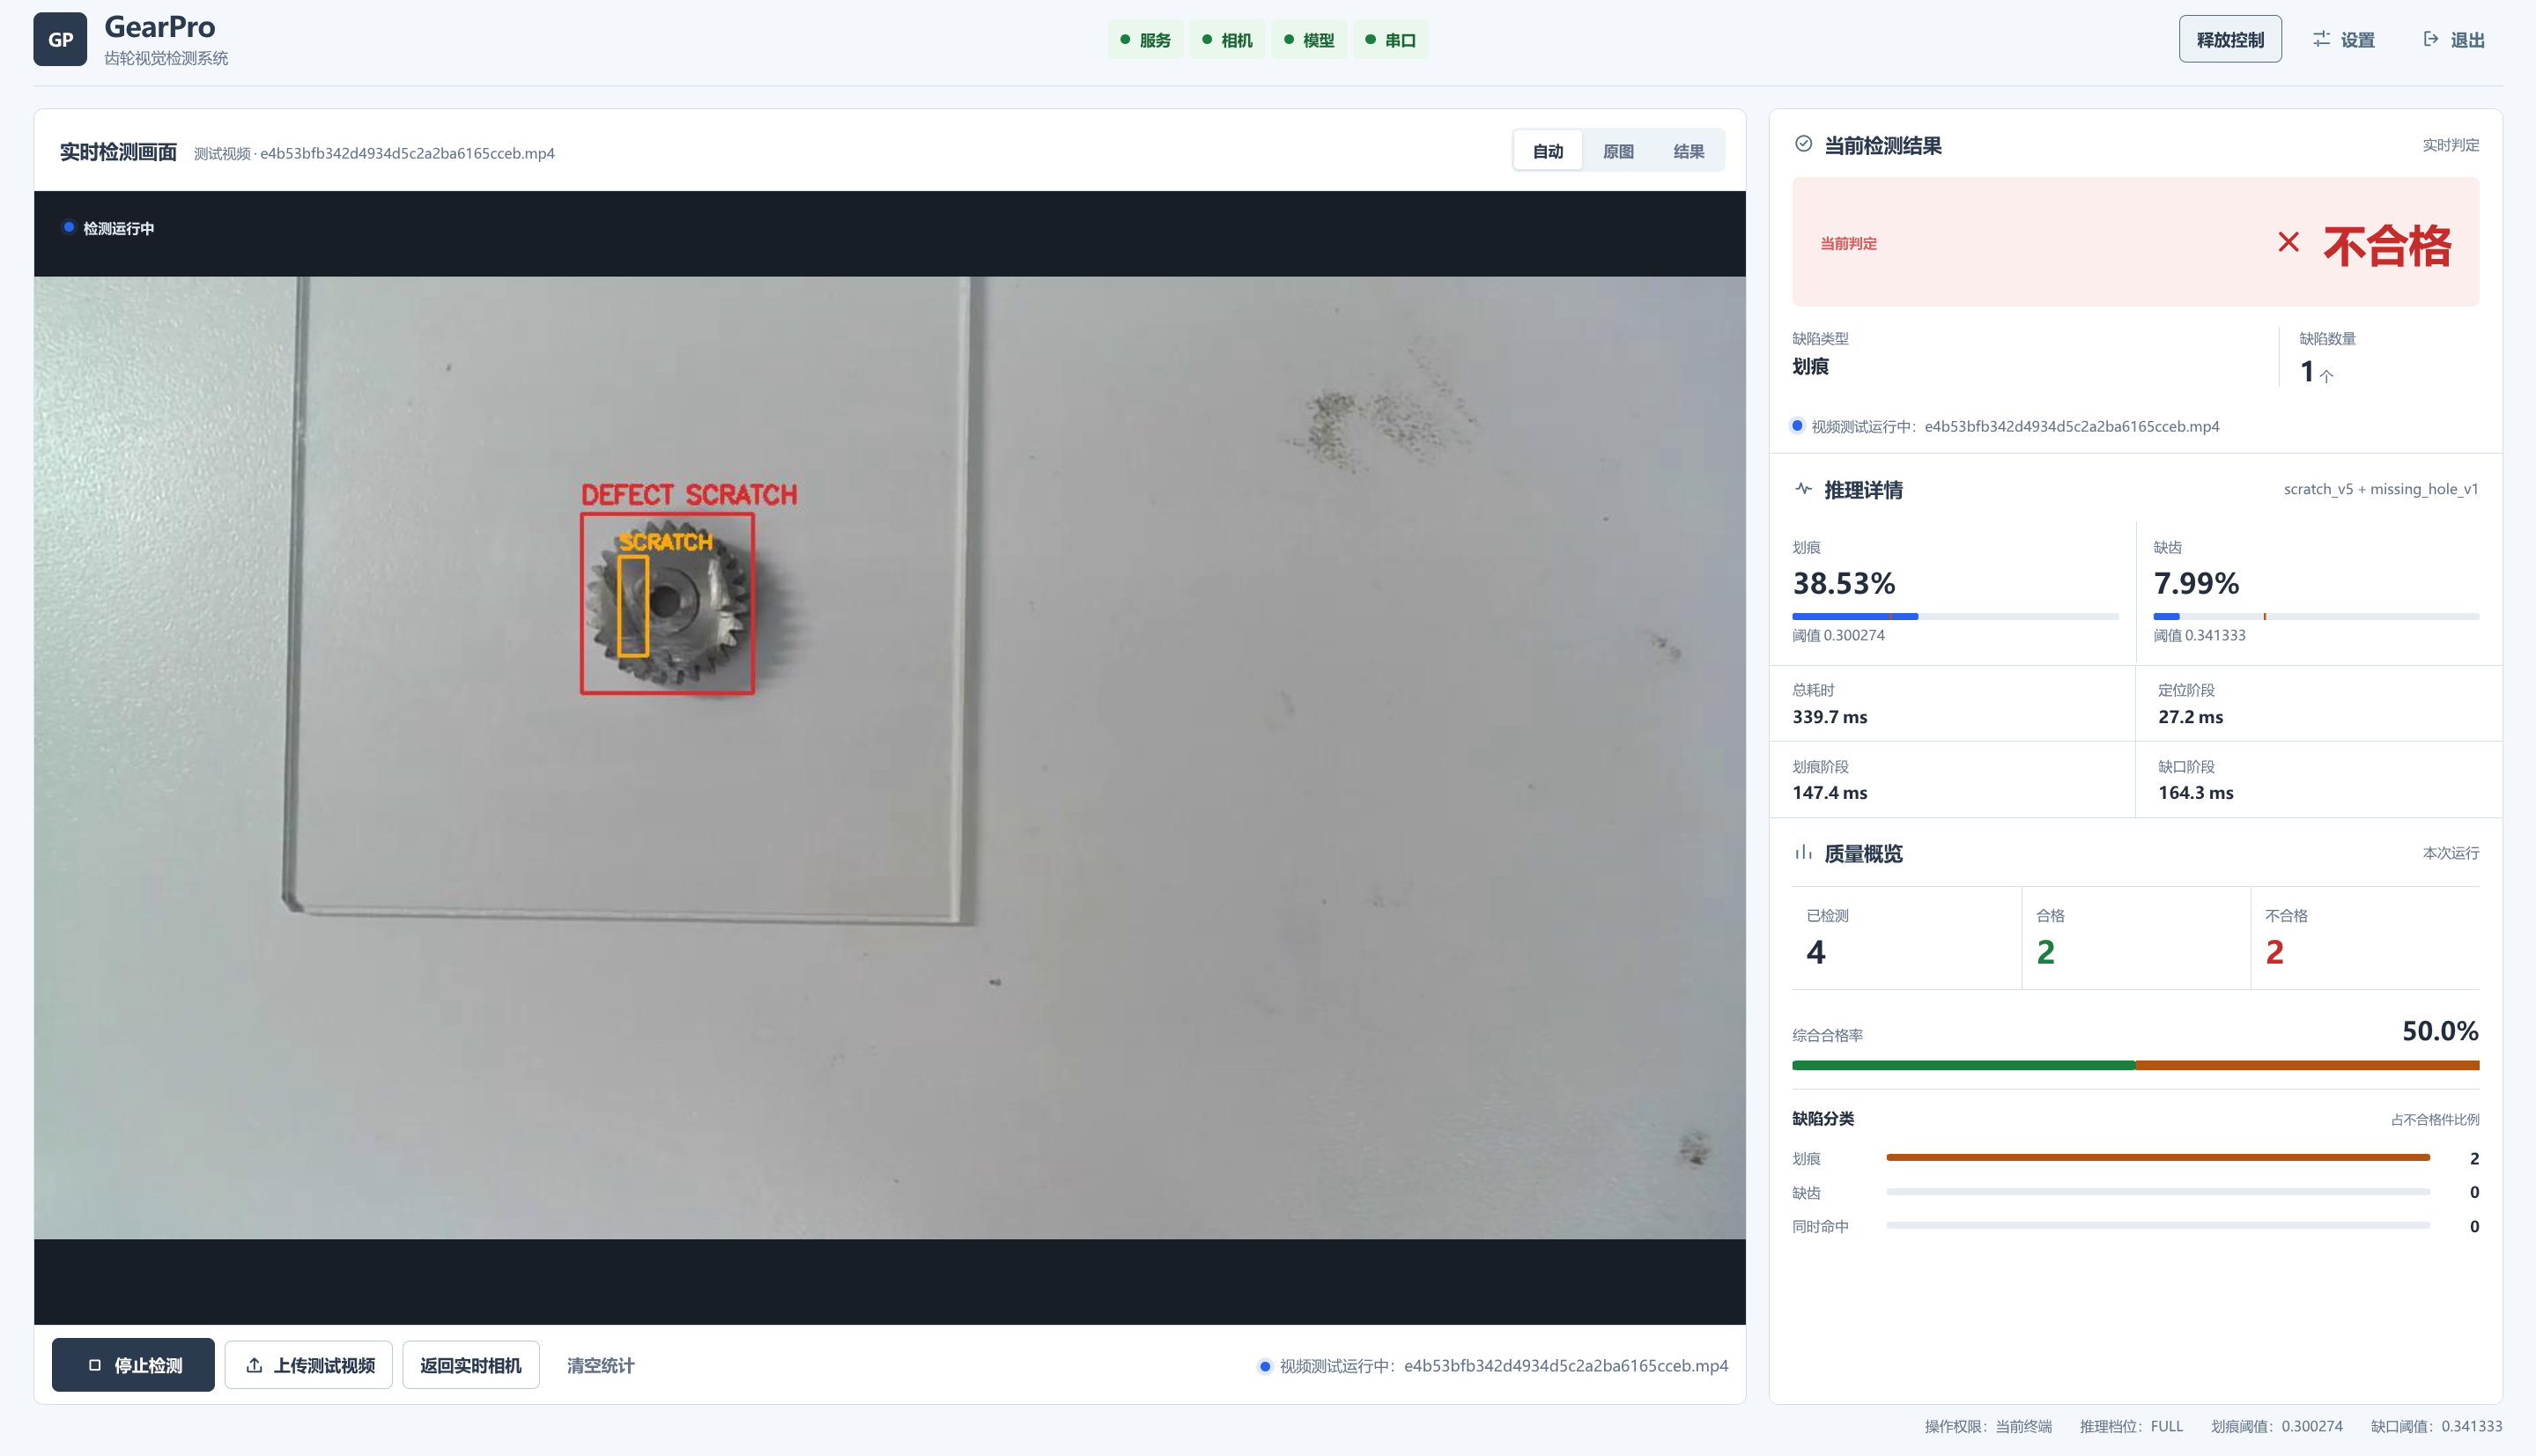
\includegraphics[width=\linewidth,height=.61\textheight,keepaspectratio]{pic/gearpro/web_console.png}
      \smallnote{现有 Web 控制台截图，后续可替换原始高分辨率版本}
    \end{column}
  \end{columns}

  \vfill
  \centering
  \textcolor{seugreen}{\large 结论：整套软件流程已运行，模型和真实设备尚未完成生产验收}
\end{frame}

% 5. Tasks and metrics
\begin{frame}{任务与评价标准}
  \begin{columns}[T,onlytextwidth]
    \begin{column}{.49\textwidth}
      {\large\bfseries 三个视觉任务}

      \vspace{.55em}
      \textbf{定位}\par
      Model1 找到齿轮位置，并产生 ROI。

      \vspace{.45em}
      \textbf{划痕}\par
      识别低对比、局部纹理型缺陷。

      \vspace{.45em}
      \textbf{缺口}\par
      识别齿形和轮廓的结构变化。

      \vspace{.5em}
      \begin{exampleblock}{最终结果怎样计算}
        从原始画面开始统计。没找到齿轮、裁剪位置偏了，或结果没有成功送出，都算检测失败。
      \end{exampleblock}
    \end{column}
    \begin{column}{.47\textwidth}
      {\large\bfseries 评价指标}

      \vspace{.55em}
      \renewcommand{\arraystretch}{1.35}
      \begin{tabularx}{\linewidth}{>{\bfseries\color{seugreen}}l X}
        Recall & 真实缺陷中被检出的比例，反映漏检风险 \\
        FPR & 正常样本被误判为缺陷的比例，反映误剔除风险 \\
        Precision & 判为缺陷的结果中真正缺陷的比例 \\
        mAP & 辅助框质量，不直接等于工件判定能力 \\
      \end{tabularx}

      \vspace{.8em}
      \centering
      {\color{seugreen}\large\bfseries 阶段目标}

      \vspace{.25em}
      {\Large Recall $\geq 0.95$}\qquad
      {\Large FPR $\leq 0.20$}
    \end{column}
  \end{columns}
\end{frame}

% 6. Pipeline
\subsection{流程与数据}
\SoftwareNav{2}
\GearProSetMinorProgressRange{6}{3}
\begin{frame}{当前视觉处理流程}
  \centering
  \resizebox{.96\textwidth}{!}{%
    \begin{tikzpicture}[node distance=.65cm and .6cm]
      \node[flow] (input) {相机或\\测试视频};
      \node[flow,right=of input] (loc) {Model1\\齿轮定位};
      \node[flow,right=of loc] (roi) {定位框外扩 4\%\\裁剪 ROI};
      \node[flowwide,right=of roi] (spec) {Scratch V5\\Missing Hole V1};
      \node[decision,right=of spec] (judge) {各自校准\\独立过阈值};
      \node[decision,right=of judge] (or) {最终 OR\\合格或剔除};
      \draw[line] (input) -- (loc);
      \draw[line] (loc) -- (roi);
      \draw[line] (roi) -- (spec);
      \draw[line] (spec) -- (judge);
      \draw[line] (judge) -- (or);
    \end{tikzpicture}%
  }

  \vspace{1.0em}
  \begin{columns}[T,onlytextwidth]
    \begin{column}{.31\textwidth}
      \textbf{多个齿轮}

      逐个生成 ROI，任意齿轮命中任意专项，整帧判为不合格。
    \end{column}
    \begin{column}{.31\textwidth}
      \textbf{没有齿轮}

      不计数，不发送串口结果，避免无效输出。
    \end{column}
    \begin{column}{.31\textwidth}
      \textbf{测试视频}

      主动禁用串口，防止测试素材触发真实执行机构。
    \end{column}
  \end{columns}

  \vfill
  \centering
  同一推理结果同时进入 \textbf{Web、统计和串口}，各模块不重复计算判定。
\end{frame}

% 7. Data split
\begin{frame}{数据拆分与锁定测试}
  \centering
  \begin{tikzpicture}[node distance=1.15cm]
    \node[flowwide] (train) {训练集\\更新模型参数};
    \node[flowwide,right=of train] (val) {验证集\\选择结构、校准与阈值};
    \node[decision,right=of val] (test) {锁定测试\\配置确定后只使用一次};
    \draw[line] (train) -- (val);
    \draw[line] (val) -- (test);
  \end{tikzpicture}

  \vspace{1em}
  \begin{columns}[T,onlytextwidth]
    \begin{column}{.48\textwidth}
      \textbf{为什么不能随机按图片拆分}
      \begin{itemize}
        \item 连续帧和相近角度高度相似
        \item 同一工件纹理可能跨集合出现
        \item 验证分数会虚高
      \end{itemize}
    \end{column}
    \begin{column}{.48\textwidth}
      \textbf{当前隔离方法}
      \begin{itemize}
        \item SHA256 检查精确重复
        \item dHash 发现视觉近似项
        \item 结合序号、宽高比和灰度相关性建组
        \item 同组不跨训练、验证和测试集合
      \end{itemize}
    \end{column}
  \end{columns}

  \vfill
  \begin{alertblock}{锁定测试的使用规则}
    锁定测试只用于最终检查。结果一旦查看，就不再用这批数据调整温度、融合权重或阈值。
  \end{alertblock}
\end{frame}

% 8. Difficult labels
\begin{frame}{Difficult 样本处理}
  \begin{columns}[T,onlytextwidth]
    \begin{column}{.46\textwidth}
      \begin{block}{保留 difficult 样本}
        保留 difficult 框，让训练集包含全部已标注缺陷。
      \end{block}

      \vspace{.55em}
      \begin{block}{排除 difficult 样本}
        删除 difficult 框；若一张图片只剩 difficult 缺陷，则整张图片退出训练。
      \end{block}
    \end{column}
    \begin{column}{.49\textwidth}
      \textbf{必须避免的错误}

      \vspace{.5em}
      \begin{alertblock}{假负样本}
        删除缺陷框后继续把图片当作正常样本，会让模型把真实缺陷学习成正常外观。
      \end{alertblock}

      \vspace{.55em}
      \textbf{统一评价}
      \begin{itemize}
        \item 验证集和测试集保留完整真值
        \item 不同训练方法使用相同的评价方式
        \item 结果显示斜视角度才是主要问题
      \end{itemize}
    \end{column}
  \end{columns}

  \vfill
  \centering
  \textcolor{seugreen}{\large 数据处理同时避免图像泄漏和错误标签含义}
\end{frame}

% 9. ROI
\subsection{架构决策}
\SoftwareNav{3}
\GearProSetMinorProgressRange{9}{2}
\begin{frame}{关键决策一：先定位，再识别缺陷}
  \begin{columns}[T,onlytextwidth]
    \begin{column}{.45\textwidth}
      \centering
      \begin{tikzpicture}
        \node[flowwide,text width=3.8cm,minimum height=2.1cm] (full) {整张图直接缩放\\背景占去大量像素\\划痕细节随之变少};
        \node[decision,text width=3.8cm,below=1.0cm of full,minimum height=1.55cm] (loss) {多次下采样后\\缺陷特征可能丢失};
        \draw[line] (full) -- (loss);
      \end{tikzpicture}
    \end{column}
    \begin{column}{.08\textwidth}
      \centering\vspace{2.4em}{\color{seugold}\Huge$\Rightarrow$}
    \end{column}
    \begin{column}{.45\textwidth}
      \centering
      \begin{tikzpicture}
        \node[flowwide,text width=3.8cm,minimum height=2.1cm] (loc) {先用 Model1 定位\\四周外扩 4\%};
        \node[flowwide,text width=3.8cm,below=1.0cm of loc,minimum height=1.55cm] (roi) {只裁出齿轮区域\\保留表面和边缘细节};
        \draw[line] (loc) -- (roi);
      \end{tikzpicture}
    \end{column}
  \end{columns}

  \vfill
  \begin{columns}[T,onlytextwidth]
    \begin{column}{.48\textwidth}
      \textbf{好处：}减少背景和摆放角度的干扰，让更多像素用于显示齿轮。
    \end{column}
    \begin{column}{.48\textwidth}
      \textbf{需要注意：}Model1 没找到齿轮仍算漏检，4\% 外扩还要在真实设备上验证。
    \end{column}
  \end{columns}
\end{frame}

% 10. Unified versus specialists
\begin{frame}{关键决策二：统一模型转向双专项}
  \begin{columns}[T,onlytextwidth]
    \begin{column}{.43\textwidth}
      \centering
      {\large\bfseries 统一模型}

      \vspace{.7em}
      \begin{tabular}{lr}
        Recall & 0.7606 \\
        FPR & 0.4177 \\
      \end{tabular}

      \vspace{1.0em}
      同时识别细小划痕和结构缺口，两类特征差别较大，当前模型难以兼顾。
    \end{column}
    \begin{column}{.12\textwidth}
      \centering\vspace{2em}{\color{seugold}\Huge$\Rightarrow$}
    \end{column}
    \begin{column}{.43\textwidth}
      \centering
      {\large\bfseries 双专项 OR}

      \vspace{.7em}
      \begin{tabular}{lr}
        Recall & \textbf{0.8873} \\
        FPR & \textbf{0.2278} \\
      \end{tabular}

      \vspace{1.0em}
      两类缺陷分别选择输入尺寸、检测结构和判断阈值。
    \end{column}
  \end{columns}

  \vfill
  \begin{block}{为什么分成两个模型}
    划痕主要是小面积、低对比的纹理变化，缺齿缺口主要改变轮廓。当前分开识别效果更好，数据增加后仍可重新比较统一模型。
  \end{block}
\end{frame}

% 11. Scratch architecture
\subsection{双专项}
\SoftwareNav{4}
\GearProSetMinorProgressRange{11}{5}
\begin{frame}{Scratch V5：整体分类与局部检测互补}
  \centering
  \resizebox{.92\textwidth}{!}{%
    \begin{tikzpicture}[node distance=.55cm and .65cm]
      \node[flowwide] (roi) {齿轮 ROI};
      \node[flowwide,above right=.15cm and 1.2cm of roi] (eff) {EfficientNet-B0\\384 输入};
      \node[flowwide,right=1.2cm of roi] (res) {ResNet18\\384 输入};
      \node[flowwide,below right=.15cm and 1.2cm of roi] (det) {YOLO26-P2\\960 输入};
      \node[decision,right=1.25cm of res] (cal) {校正三路分数};
      \node[decision,right=1.0cm of cal] (fuse) {得到综合分数};
      \draw[line] (roi) -- (eff);
      \draw[line] (roi) -- (res);
      \draw[line] (roi) -- (det);
      \draw[line] (eff.east) -- (cal.west);
      \draw[line] (res) -- (cal);
      \draw[line] (det.east) -- (cal.west);
      \draw[line] (cal) -- (fuse);
    \end{tikzpicture}%
  }

  \vspace{.7em}
  \begin{exampleblock}{最终分数计算}
    \centering
    $p_{\mathrm{scratch}} = 0.25\,p_{\mathrm{cls}} + 0.75\,p_{\mathrm{det}}$
    \qquad
    阈值 $= 0.300273610279458$
  \end{exampleblock}

  \vfill
  \begin{columns}[T,onlytextwidth]
    \begin{column}{.48\textwidth}
      两个分类器判断整张齿轮图像，P2 检测器重点寻找细小划痕。
    \end{column}
    \begin{column}{.48\textwidth}
      较低的检测分数也参与最终计算；画框使用更高门槛，只供人工查看。
    \end{column}
  \end{columns}
\end{frame}

% 12. Scratch result
\begin{frame}{Scratch V5 锁定测试结果}
  \begin{columns}[T,onlytextwidth]
    \begin{column}{.39\textwidth}
      \centering
      % TODO: replace with the original high-resolution scratch image when available.
      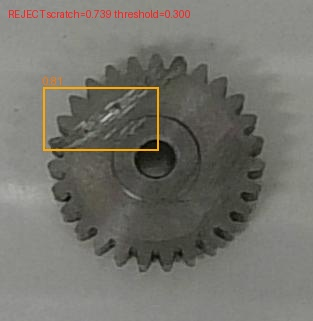
\includegraphics[width=.82\linewidth,height=.59\textheight,keepaspectratio]{pic/gearpro/scratch_reject.jpg}
      \smallnote{现有划痕检测示例}
    \end{column}
    \begin{column}{.57\textwidth}
      \vspace{.3em}
      \begin{columns}[T,onlytextwidth]
        \begin{column}{.32\textwidth}
          \centering {\color{seugreen}\LARGE\bfseries 0.8065}\\Recall
        \end{column}
        \begin{column}{.32\textwidth}
          \centering {\color{seugreen}\LARGE\bfseries 0.5556}\\Precision
        \end{column}
        \begin{column}{.32\textwidth}
          \centering {\color{seugreen}\LARGE\bfseries 0.1681}\\FPR
        \end{column}
      \end{columns}

      \vspace{1.0em}
      \centering
      \begin{tabular}{ccccc}
        \toprule
        样本 & TP & FP & TN & FN \\
        \midrule
        150 & 25 & 20 & 99 & 6 \\
        \bottomrule
      \end{tabular}

      \vspace{1em}
      \begin{itemize}
        \item 漏检（FN）：颜色浅、面积小或形态不稳定的划痕
        \item 误报（FP）：侧齿高光和正常加工纹
      \end{itemize}
    \end{column}
  \end{columns}

  \vfill
  \centering
  \textcolor{seugreen}{局部检测器更容易发现细小划痕，但仍会把高光和正常加工纹看成缺陷}
\end{frame}

% 13. Missing architecture
\begin{frame}{Missing Hole V1：结构缺陷专项}
  \centering
  \resizebox{.92\textwidth}{!}{%
    \begin{tikzpicture}[node distance=.55cm and .65cm]
      \node[flowwide] (roi) {齿轮 ROI};
      \node[flowwide,above right=.15cm and 1.2cm of roi] (eff) {EfficientNet-B0\\512 输入};
      \node[flowwide,right=1.2cm of roi] (res) {ResNet18\\384 输入};
      \node[flowwide,below right=.15cm and 1.2cm of roi] (det) {标准 YOLO26n\\960 输入};
      \node[decision,right=1.25cm of res] (cal) {校正三路分数};
      \node[decision,right=1.0cm of cal] (fuse) {得到综合分数};
      \draw[line] (roi) -- (eff);
      \draw[line] (roi) -- (res);
      \draw[line] (roi) -- (det);
      \draw[line] (eff.east) -- (cal.west);
      \draw[line] (res) -- (cal);
      \draw[line] (det.east) -- (cal.west);
      \draw[line] (cal) -- (fuse);
    \end{tikzpicture}%
  }

  \vspace{.7em}
  \begin{exampleblock}{最终分数计算}
    \centering
    $p_{\mathrm{missing}} = 0.50\,p_{\mathrm{cls}} + 0.50\,p_{\mathrm{det}}$
    \qquad
    阈值 $= 0.3413327979078584$
  \end{exampleblock}

  \vfill
  \begin{block}{为什么没有使用 P2}
    在 Missing Hole 验证中，P2 没有稳定优于标准检测结构，因此采用结果更稳定、结构更简单的方案。
  \end{block}
\end{frame}

% 14. Missing result
\begin{frame}{Missing Hole V1 锁定测试结果}
  \begin{columns}[T,onlytextwidth]
    \begin{column}{.36\textwidth}
      \centering
      % TODO: replace with the original high-resolution oblique image when available.
      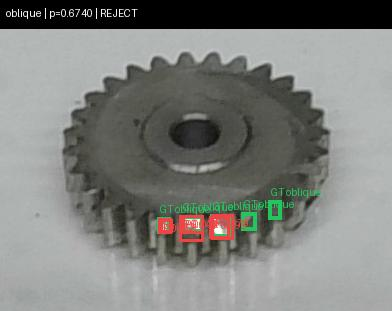
\includegraphics[width=.9\linewidth,height=.54\textheight,keepaspectratio]{pic/gearpro/oblique_missing.jpg}
      \smallnote{斜视（oblique）缺口示例}
    \end{column}
    \begin{column}{.6\textwidth}
      \begin{columns}[T,onlytextwidth]
        \begin{column}{.32\textwidth}
          \centering {\color{seugreen}\LARGE\bfseries 0.8182}\\Recall
        \end{column}
        \begin{column}{.32\textwidth}
          \centering {\color{seugreen}\LARGE\bfseries 0.9000}\\Precision
        \end{column}
        \begin{column}{.32\textwidth}
          \centering {\color{seugreen}\LARGE\bfseries 0.0377}\\FPR
        \end{column}
      \end{columns}

      \vspace{.8em}
      \textbf{不同位置的 Recall}

      \vspace{.35em}
      \begin{tabular}{@{}l@{\hspace{.8em}}l@{\hspace{.8em}}r@{}}
        bottom & \textcolor{seugreen}{\rule{3.20cm}{1.1ex}} & 0.9167 \\
        side & \textcolor{seugreen}{\rule{3.49cm}{1.1ex}} & 1.0000 \\
        oblique & \textcolor{seugold}{\rule{2.05cm}{1.1ex}} & \textbf{0.5882} \\
      \end{tabular}

      \vspace{.8em}
      TP/FP/TN/FN：36/4/102/8
    \end{column}
  \end{columns}

  \vfill
  \begin{alertblock}{当前主要问题}
    是否计入 difficult 样本对结果影响很小。斜视角度下缺口不够清楚，才是当前最明显的问题。
  \end{alertblock}
\end{frame}

% 15. OR decision
\begin{frame}{关键决策三：两个模型分别判断后再合并}
  \centering
  \begin{tikzpicture}[node distance=1.1cm and 1.05cm]
    \node[flowwide,text width=3.75cm] (scratch) {Scratch 概率\\{\scriptsize$\geq 0.300273610279458$}};
    \node[flowwide,text width=3.75cm,below=of scratch] (missing) {Missing Hole 概率\\{\scriptsize$\geq 0.3413327979078584$}};
    \coordinate (join) at ($(scratch.east)!0.5!(missing.east)+(0.75cm,0)$);
    \node[decision,right=1.0cm of join] (or) {任一模型判为缺陷};
    \node[flowwide,right=1.25cm of or] (final) {最终结果\\合格或不合格};
    \draw[very thick,draw=seugreen] (scratch.east) -| (join);
    \draw[very thick,draw=seugreen] (missing.east) -| (join);
    \draw[line] (join) -- (or.west);
    \draw[line] (or) -- (final);
  \end{tikzpicture}

  \vspace{1em}
  \begin{columns}[T,onlytextwidth]
    \begin{column}{.47\textwidth}
      \textbf{为什么分别判断}

      两个模型识别的缺陷不同，分数范围也不同，不能直接相加后使用同一个阈值。
    \end{column}
    \begin{column}{.47\textwidth}
      \textbf{合并后的影响}

      一个模型可以补回另一个模型漏掉的缺陷，但两个模型的误报也会累积。
    \end{column}
  \end{columns}

  \vfill
  \centering
  同一齿轮同时命中两个专项时保留两个原因，统计和串口只输出一次。
\end{frame}

% 16. Core results
\subsection{结果与工程}
\SoftwareNav{5}
\GearProSetMinorProgressRange{16}{13}
\begin{frame}{核心锁定测试结果}
  \centering
  \renewcommand{\arraystretch}{1.3}
  \begin{tabular}{lrrrr}
    \toprule
    方案 & Recall & Precision & FPR & TP/FP/TN/FN \\
    \midrule
    Scratch V5 专项 & 0.8065 & 0.5556 & 0.1681 & 25/20/99/6 \\
    Missing Hole V1 专项 & 0.8182 & 0.9000 & 0.0377 & 36/4/102/8 \\
    \rowcolor{seuyellowlight}
    双专项 OR & \textbf{0.8873} & \textbf{0.7778} & \textbf{0.2278} & 63/18/61/8 \\
    统一 EfficientNet-B0 & 0.7606 & 0.6207 & 0.4177 & 54/33/46/17 \\
    \bottomrule
  \end{tabular}

  \vspace{1.2em}
  \begin{columns}[T,onlytextwidth]
    \begin{column}{.47\textwidth}
      \textbf{同一批数据下的结果}

      两个模型合并后比统一模型少漏检，正常件误报也明显减少。
    \end{column}
    \begin{column}{.47\textwidth}
      \textbf{需要注意的数字}

      两个模型使用的正常样本范围不同，各自的 FPR 不能直接相加。
    \end{column}
  \end{columns}

  \vfill
  \centering
  \textcolor{seugreen}{当前方案优于统一模型，但仍未达到生产目标}
\end{frame}

% 17. Target gap
\begin{frame}{目标差距与阈值使用规则}
  \begin{columns}[T,onlytextwidth]
    \begin{column}{.48\textwidth}
      \centering
      {\small Recall}

      \vspace{.25em}
      {\color{seugreen}\Huge\bfseries 0.8873}

      \vspace{.15em}
      目标 0.95，仍差 \textbf{0.0627}
    \end{column}
    \begin{column}{.48\textwidth}
      \centering
      {\small FPR}

      \vspace{.25em}
      {\color{seugreen}\Huge\bfseries 0.2278}

      \vspace{.15em}
      上限 0.20，超出 \textbf{0.0278}
    \end{column}
  \end{columns}

  \vspace{1em}
  \begin{alertblock}{不能继续用当前测试集调整阈值}
    这批数据已经用于最终检查。如果看过结果后继续调阈值，得到的提升可能只适用于这批数据，还可能明显增加误报。
  \end{alertblock}

  \vfill
  \centering
  下一轮应使用新数据选择模型和阈值，确定后再建立一批从未用于调整的新测试数据。
\end{frame}

% 18. Error patterns
\begin{frame}{主要错误模式}
  \begin{columns}[T,onlytextwidth]
    \begin{column}{.31\textwidth}
      \textbf{浅划痕漏检}

      缺陷纹理接近正常加工纹。优先稳定低角度照明，并补采真实弱划痕。
    \end{column}
    \begin{column}{.31\textwidth}
      \textbf{斜视缺口漏检}

      单一视角下结构变化不稳定。优先验证背光、第二相机或转台。
    \end{column}
    \begin{column}{.31\textwidth}
      \textbf{高光正常件误报}

      侧齿反光和加工纹触发划痕分支。需要调整光源并扩充真实负样本。
    \end{column}
  \end{columns}

  \vspace{.85em}
  \centering
  % TODO: replace this montage with original full-resolution error cases when available.
  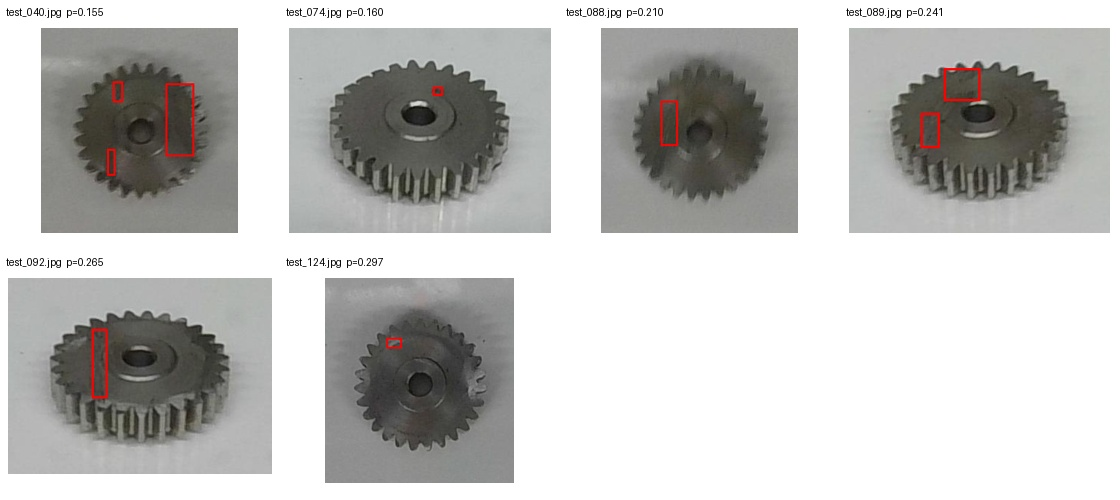
\includegraphics[width=.88\linewidth,height=.42\textheight,keepaspectratio]{pic/gearpro/error_cases.jpg}
  \smallnote{现有错误样本组合图，后续替换为原始单图}
\end{frame}

% 19. Error-analysis conclusion
\begin{frame}{软件结果的当前判断}
  \begin{columns}[T,onlytextwidth]
    \begin{column}{.31\textwidth}
      \centering
      {\color{seugreen}\Large\bfseries 实验}

      \vspace{.5em}
      已避免相似图片跨集合，并建立锁定测试和 Recall/FPR 双重要求。
    \end{column}
    \begin{column}{.31\textwidth}
      \centering
      {\color{seugreen}\Large\bfseries 模型}

      \vspace{.5em}
      已形成 Model1 定位与 Scratch、Missing Hole 双专项方案。
    \end{column}
    \begin{column}{.31\textwidth}
      \centering
      {\color{seugreen}\Large\bfseries 差距}

      \vspace{.5em}
      联合 Recall 0.8873、FPR 0.2278，真实设备结果仍待验收。
    \end{column}
  \end{columns}

  \vspace{1.1em}
  \begin{block}{当前判断}
    浅划痕、斜视缺口和高光误报都与图像是否看得清、样本是否覆盖充分有关。下一阶段先验证成像条件，再决定是否需要更复杂的模型。
  \end{block}

  \vfill
  \begin{exampleblock}{后续软件内容}
    继续说明实时架构、模型发布、现场演示与优化路线，再进入硬件结构和联合验收。
  \end{exampleblock}
\end{frame}

% 20. Runtime architecture
\subsection{结果与工程}
\SoftwareNav{5}
\begin{frame}{软件如何持续处理实时画面}
  \centering
  \begin{tikzpicture}[node distance=.35cm]
    \node[flow,text width=1.9cm,inner sep=3pt] (camera) {Camera\\Capture\\只保留最新帧};
    \node[flow,text width=1.8cm,inner sep=3pt,right=of camera] (latest) {Latest\\Frame\\交付最新图像};
    \node[flow,text width=1.95cm,inner sep=3pt,right=of latest] (worker) {Inspection\\Worker\\独立线程推理};
    \node[decision,text width=1.85cm,inner sep=3pt,right=of worker] (result) {Observation\\唯一结果对象};
    \node[flow,text width=2.0cm,inner sep=3pt,right=of result] (output) {Web、统计\\串口输出};
    \draw[line] (camera) -- (latest);
    \draw[line] (latest) -- (worker);
    \draw[line] (worker) -- (result);
    \draw[line] (result) -- (output);
  \end{tikzpicture}

  \vspace{1.1em}
  \begin{columns}[T,onlytextwidth]
    \begin{column}{.47\textwidth}
      \textbf{后台处理方式}
      \begin{itemize}
        \item 图像采集和模型计算在独立后台线程运行
        \item 暂停、恢复和浏览器重连复用已加载模型
        \item 原图与标注图各保存一份，多台浏览器直接共用
      \end{itemize}
    \end{column}
    \begin{column}{.47\textwidth}
      \textbf{页面使用方式}
      \begin{itemize}
        \item 最新帧优先，避免排队造成结果滞后
        \item 浏览器只负责查看和控制，不拥有检测任务
        \item 页面刷新或临时断线不终止后台检测
      \end{itemize}
    \end{column}
  \end{columns}
\end{frame}

% 21. Bounded modes
\begin{frame}{运行档位与异常保护}
  \renewcommand{\arraystretch}{1.25}
  \begin{tabularx}{\linewidth}{>{\bfseries}l X X}
    \toprule
    档位 & 当前行为 & 适用条件 \\
    \midrule
    FULL & 运行完整定位与双专项链路 & 正常检测与正式测试 \\
    SPARSE & 增加推理间隔，模型组成不变 & 资源或温度压力较高 \\
    SAFE\_STOP & 停止检测，不继续输出有效结果 & 必要模块失败或状态非法 \\
    \bottomrule
  \end{tabularx}

  \vspace{1em}
  \begin{block}{出现这些异常时停止检测}
    必要模型未加载、没有有效齿轮区域、模型文件校验失败、计算结果异常或显存不足时停止检测。尚未实现的档位必须明确显示“不可用”。
  \end{block}

  \vfill
  SystemSnapshot v2 汇总系统、相机、模型、串口和任务状态。当前可以查看状态并在部分异常下安全停机，但还不能自动处理所有故障。
\end{frame}

% 22. Model package
\begin{frame}{模型发布包：配置与文件一一对应}
  \begin{columns}[T,onlytextwidth]
    \begin{column}{.44\textwidth}
      \begin{block}{配置清单记录的内容}
        \begin{itemize}
          \item 版本、模型类型与输入尺寸
          \item 预处理、温度与融合权重
          \item 判断阈值和模型文件位置
          \item 模型文件校验值与对应代码版本
        \end{itemize}
      \end{block}
    \end{column}
    \begin{column}{.51\textwidth}
      \begin{exampleblock}{启动时检查}
        \begin{itemize}
          \item 配置与权重不匹配时拒绝启动
          \item 分类器从本地加载模型文件，不依赖在线下载
          \item 加载后先试运行一次，尽早发现错误
          \item 分数校正参数、融合比例和阈值固定在版本内
        \end{itemize}
      \end{exampleblock}
    \end{column}
  \end{columns}

  \vfill
  \centering
  \textcolor{seugreen}{\large 每次结果都能对应到具体配置和模型文件，才能稳定复现}
\end{frame}

% 23. Single source of truth
\begin{frame}{一次检测，页面、统计和串口共用同一结果}
  \centering
  \begin{tikzpicture}[node distance=.75cm]
    \node[decision,text width=3.6cm] (obs) {Observation\\定位置信度、专项概率、实际阈值\\分支概率、辅助框、拒绝原因、耗时};
    \node[flow,right=1.15cm of obs,yshift=1.25cm] (web) {Web 展示};
    \node[flow,right=1.15cm of obs] (stats) {运行统计};
    \node[flow,right=1.15cm of obs,yshift=-1.25cm] (serial) {串口输出};
    \draw[line] (obs.east) -- ++(.5,0) |- (web.west);
    \draw[line] (obs.east) -- (stats.west);
    \draw[line] (obs.east) -- ++(.5,0) |- (serial.west);
  \end{tikzpicture}

  \vspace{.8em}
  \begin{columns}[T,onlytextwidth]
    \begin{column}{.47\textwidth}
      \textbf{结果保持一致}

      页面、统计和串口不各自重复判断。阈值改变后，已有记录保持不变。
    \end{column}
    \begin{column}{.47\textwidth}
      \textbf{谁可以操作}

      多台设备可以同时查看，但一次只允许一个已登录会话操作，操作权保持 30 秒。修改设置、切换数据源和启停检测都需要操作权。
    \end{column}
  \end{columns}

  \vfill
  \small 当前网页服务只适合可信的独立局域网；如果跨网段或接入公网，需要额外配置 HTTPS 和访问保护。
\end{frame}

% 24. Demo
\begin{frame}{现场演示流程与能说明的范围}
  \begin{columns}[T,onlytextwidth]
    \begin{column}{.58\textwidth}
      \renewcommand{\arraystretch}{1.18}
      \begin{tabular}{>{\bfseries\color{seugreen}}r p{6.1cm}}
        1 & 启动 Jetson 服务并完成模型预热 \\
        2 & 检查服务、相机、模型和串口状态 \\
        3 & 获取操作权，启动实时相机 \\
        4 & 上传固定视频，依次展示正常与两类缺陷 \\
        5 & 核对概率、阈值、拒绝原因、耗时和统计 \\
        6 & 验证视频模式禁用串口，再返回实时相机 \\
      \end{tabular}
    \end{column}
    \begin{column}{.37\textwidth}
      \begin{block}{现场备份}
        录屏、截图和本地固定视频。
      \end{block}
      \begin{alertblock}{边界}
        演示只能说明整套功能可以运行，不能代替生产条件下的性能验收。现场不调阈值、不修改模型。
      \end{alertblock}
    \end{column}
  \end{columns}
\end{frame}

% 25. Imaging and data optimization
\subsection{结果与工程}
\SoftwareNav{5}
\begin{frame}{优化路线一：成像、数据与实验设计}
  \begin{columns}[T,onlytextwidth]
    \begin{column}{.47\textwidth}
      \textbf{先固定输入条件}
      \begin{itemize}
        \item 记录工作距离、焦距、曝光、照明与姿态
        \item 补采弱划痕正样本和高光、加工纹、灰尘、轻微失焦负样本
        \item 对缺口比较低角度光、背光和补充视角
      \end{itemize}
    \end{column}
    \begin{column}{.47\textwidth}
      \textbf{再统一实验方法}
      \begin{itemize}
        \item 同一工件的连续帧、不同照明和视角归入同一组
        \item 图像增强只模拟现场可能变化，并确保最小缺陷仍看得见
        \item 每轮只改变一个主要变量，同时报告总体与关键子组
      \end{itemize}
    \end{column}
  \end{columns}

  \vfill
  \begin{block}{判断顺序}
    先确认原始图像是否包含足够缺陷信息，再决定重新训练、调整阈值或增加模型复杂度。
  \end{block}
\end{frame}

% 26. Geometry and model experiments
\begin{frame}{优化路线二：齿轮位置校正与模型对比}
  \begin{columns}[T,onlytextwidth]
    \begin{column}{.45\textwidth}
      \begin{block}{统一齿轮位置和方向}
        \begin{itemize}
          \item 在 ROI 后估计齿轮中心和直径
          \item 比较不校正、旋转校正与极坐标展开
          \item 检查校正后是否更容易稳定识别划痕和缺口
        \end{itemize}
      \end{block}
    \end{column}
    \begin{column}{.5\textwidth}
      \begin{block}{逐项比较模型结构}
        \begin{itemize}
          \item Scratch 比较完整 P2、减通道 P2 与轻量分支
          \item 分别比较融合层数、输出通道数和注意力模块
          \item 只有精度不下降且速度提高时才删除 P5
          \item 设备算力仍不足时，再尝试用大模型指导小模型训练
        \end{itemize}
      \end{block}
    \end{column}
  \end{columns}

  \vfill
  每组实验同步报告 Recall、FPR、Precision、关键子组、延迟、显存、参数量与功耗，避免同时改变多个变量后只展示最佳结果。
\end{frame}

% 27. Jetson deployment
\begin{frame}{优化路线三：Jetson 运行速度与部署}
  \centering
  \begin{tikzpicture}[node distance=.38cm]
    \node[flow,text width=2.0cm] (pt) {.pt\\当前精度与速度};
    \node[decision,text width=2.05cm,right=of pt] (m1) {Model1\\FP16 TensorRT};
    \node[flow,text width=2.0cm,right=of m1] (retest) {分项性能复测};
    \node[flow,text width=2.05cm,right=of retest] (special) {优先转换\\最耗时的模型};
    \node[flow,text width=2.05cm,right=of special] (later) {必要时评估 INT8\\剪枝与复制优化};
    \draw[line] (pt) -- (m1);
    \draw[line] (m1) -- (retest);
    \draw[line] (retest) -- (special);
    \draw[line] (special) -- (later);
  \end{tikzpicture}

  \vspace{1em}
  \begin{columns}[T,onlytextwidth]
    \begin{column}{.47\textwidth}
      \textbf{分步骤记录耗时}

      分开记录取帧、定位、分类、检测、结果合并、绘图和网页传输的耗时，同时记录每秒处理量、显存、功耗和温度。
    \end{column}
    \begin{column}{.47\textwidth}
      \textbf{部署时需要注意}

      TensorRT 文件与 GPU、JetPack 和 TensorRT 版本相关，必须在目标 NX 上生成。使用 INT8 前要准备独立校准数据，并完整比较转换前后的精度。
    \end{column}
  \end{columns}
\end{frame}

% 28. Software conclusion
\begin{frame}{软件阶段结论}
  \begin{columns}[T,onlytextwidth]
    \begin{column}{.23\textwidth}
      \centering\textbf{实验}\par\vspace{.4em}
      已避免相似图片跨集合，并建立锁定测试和 Recall/FPR 双重要求。
    \end{column}
    \begin{column}{.23\textwidth}
      \centering\textbf{模型}\par\vspace{.4em}
      Model1 与 Scratch、Missing Hole 两个专项已经形成当前对照方案。
    \end{column}
    \begin{column}{.23\textwidth}
      \centering\textbf{工程}\par\vspace{.4em}
      模型文件、后台处理、网页、统计和串口已经连通，结果可以追溯。
    \end{column}
    \begin{column}{.23\textwidth}
      \centering\textbf{差距}\par\vspace{.4em}
      Recall 0.8873、FPR 0.2278，真实设备数据尚未完成。
    \end{column}
  \end{columns}

  \vspace{1.1em}
  \begin{block}{进入硬件实验的理由}
    当前主要错误与缺陷是否拍得清楚、样本是否覆盖充分有关。下一阶段先固定成像条件，再重新比较模型和阈值。
  \end{block}
\end{frame}

% 29. Hardware goals
\section{硬件}
\subsection{平台目标}
\HardwareNav{1}
\GearProSetMinorProgressRange{29}{2}
\begin{frame}{第一代可调视觉实验平台}
  \begin{columns}[T,onlytextwidth]
    \begin{column}{.47\textwidth}
      \begin{block}{阶段定位}
        拟用万向夹固定玻璃载台、相机和光源。先验证位置、照明与摆放条件，再依据实验结果确定固定结构。
      \end{block}
      \textbf{当前状态：方案明确，实物和重复性数据待补充。}
    \end{column}
    \begin{column}{.47\textwidth}
      \textbf{设计目标}
      \begin{itemize}
        \item 完整拍摄齿轮并保留微小缺陷细节
        \item 分别验证背光轮廓和低角度表面照明
        \item 检查锁紧、重复放件和参数恢复稳定性
        \item 判断固定位置及第二相机或转台需求
      \end{itemize}
    \end{column}
  \end{columns}

  \vfill
  阶段交付包括结构照片或草图、器材参数表、空载与放件对照图，以及有实验依据的初步结构结论。
\end{frame}

% 30. Hardware layout
\begin{frame}{总体结构与空间布局}
  \centering
  \begin{tikzpicture}[node distance=.18cm]
    \node[flowwide,minimum height=.62cm,inner sep=2pt] (base) {稳定基座 / 立柱};
    \node[flowwide,minimum height=.62cm,inner sep=2pt,below=of base] (clamp) {万向夹 A};
    \node[flowwide,minimum height=.62cm,inner sep=2pt,below=of clamp] (camera) {顶部主相机};
    \node[decision,minimum height=.62cm,inner sep=2pt,below=of camera] (gear) {待测齿轮};
    \node[flowwide,minimum height=.72cm,inner sep=2pt,below=of gear] (glass) {玻璃载台\\边缘支撑与夹持};
    \node[flowwide,minimum height=.62cm,inner sep=2pt,below=of glass] (backlight) {独立支撑背光};
    \node[flow,minimum height=.72cm,inner sep=2pt,left=1.25cm of gear] (second) {第二相机\\预留区};
    \node[flow,minimum height=.72cm,inner sep=2pt,right=1.25cm of gear] (surface) {可调低角度光\\万向夹 B};
    \draw[line] (base) -- (clamp);
    \draw[line] (clamp) -- (camera);
    \draw[line] (camera) -- (gear);
    \draw[line] (gear) -- (glass);
    \draw[line] (backlight) -- (glass);
    \draw[dashed,very thick,draw=seugreen] (second) -- (gear);
    \draw[dashed,very thick,draw=seugreen] (surface) -- (gear);
  \end{tikzpicture}

  \vspace{.35em}
  \small 相机采用短悬臂，光源独立调节，夹具避开齿圈检测区；同时预留放件、清洁、走线和第二视角空间。未知型号、尺寸与载荷统一标为待确认。
\end{frame}

% 31. Camera
\subsection{相机与载台}
\HardwareNav{2}
\GearProSetMinorProgressRange{31}{2}
\begin{frame}{主相机视角与工作距离}
  \begin{columns}[T,onlytextwidth]
    \begin{column}{.43\textwidth}
      \begin{block}{基线视角}
        顶部正视，光轴基本垂直载台并平行于平放齿轮轴线。该视角便于观察完整轮廓、估计中心和尺度。
      \end{block}
      \begin{alertblock}{边界}
        顶部相机不能保证看清侧齿、遮挡区域和全部 oblique 缺口。
      \end{alertblock}
    \end{column}
    \begin{column}{.52\textwidth}
      \textbf{确定方法}
      \begin{enumerate}
        \item 纳入最大齿轮并保留摆放余量
        \item 调整距离与对焦，检查中心和边缘清晰度
        \item 核对最小缺陷在原图、齿轮裁剪图和模型输入中占多少像素
        \item 记录位置和参数，锁紧后复拍
      \end{enumerate}
      \textbf{必须记录：}镜头、测距基准、分辨率、曝光、增益、焦距、光圈、对焦状态和单位长度像素数。
    \end{column}
  \end{columns}
\end{frame}

% 32. Glass stage
\begin{frame}{玻璃载台与工件夹持}
  \begin{columns}[T,onlytextwidth]
    \begin{column}{.47\textwidth}
      \textbf{结构要求}
      \begin{itemize}
        \item 分散边缘支撑并使用合适软垫
        \item 避免长距离悬空和单点集中压紧
        \item 检测区外设置基准标记或限位件
        \item 夹持部件不得遮挡孔、端面和齿圈
        \item 玻璃规格、跨度和载荷依据实物确认
      \end{itemize}
    \end{column}
    \begin{column}{.47\textwidth}
      \textbf{光学风险}
      \begin{itemize}
        \item 上下表面反射可能形成高光
        \item 灰尘、油污和划伤可能成为伪缺陷
        \item 每组实验保留空载台图作为对照
        \item 记录清洁与更换情况
        \item 持续干扰时比较光路、玻璃或替代支撑
      \end{itemize}
    \end{column}
  \end{columns}

  \vfill
  \begin{block}{载台作用}
    玻璃同时承担工件支撑和背光透射，结构稳定与背景洁净需要同时验证。
  \end{block}
\end{frame}

% 33. Lighting
\subsection{照明方案}
\HardwareNav{3}
\GearProSetMinorProgressRange{33}{1}
\begin{frame}{背光与低角度表面照明}
  \renewcommand{\arraystretch}{1.2}
  \begin{tabularx}{\linewidth}{>{\bfseries}l X X}
    \toprule
    & 背光 & 低角度表面光 \\
    \midrule
    主要信息 & 齿轮投影轮廓，适合观察改变外轮廓的缺齿或贯通开口 & 表面高低和反光变化，适合观察浅划痕 \\
    关键变量 & 覆盖范围、距离、过曝与支撑阴影 & 高度、水平距离、仰角、方位与亮度 \\
    主要风险 & 未改变投影的局部缺口仍可能不可见 & 加工纹、灰尘、玻璃划伤和高光同步增强 \\
    验证对象 & 缺口件、正常轮廓，以及 Model1 是否仍能正常定位 & 真实划痕与加工纹明显的正常件 \\
    \bottomrule
  \end{tabularx}

  \vspace{.8em}
  \begin{block}{初期采集规则}
    同一静止工件分别采集两种照明，切换时保持相机和工件不动，并用唯一工件编号关联。自动切灯、曝光切换、跨帧配对和缺帧处理尚未实现。
  \end{block}
\end{frame}

% 34. Clamp stability
\subsection{扩展视角}
\HardwareNav{4}
\GearProSetMinorProgressRange{34}{2}
\begin{frame}{万向夹调节与重复性检查}
  \scriptsize
  \renewcommand{\arraystretch}{1.2}
  \begin{tabularx}{\linewidth}{>{\bfseries}l X X}
    \toprule
    模块 & 主要调节项目 & 锁紧后重点检查 \\
    \midrule
    主相机 & 高度、水平位置、俯仰、横滚 & 下垂、画面漂移、清晰度变化 \\
    玻璃载台 & 高度、水平度、夹持位置 & 晃动、倾斜、局部受力、遮挡 \\
    表面光源 & 高度、距离、仰角、方位 & 光照方向变化、关节松动 \\
    背光 & 水平位置、距离 & 覆盖范围、支撑阴影 \\
    \bottomrule
  \end{tabularx}

  \normalsize
  \vspace{.8em}
  \begin{columns}[T,onlytextwidth]
    \begin{column}{.58\textwidth}
      \textbf{重复性检查}
      \begin{enumerate}
        \item 结构不动时连续拍摄
        \item 取下并重新放置同一工件后复拍
        \item 调开夹具，再按记录恢复参数后复拍
      \end{enumerate}
    \end{column}
    \begin{column}{.37\textwidth}
      标尺、位置标记、角度记录和结构照片用于恢复配置。稳定性不足时先缩短悬臂、加强基座和线缆固定。
    \end{column}
  \end{columns}
\end{frame}

% 35. Extra viewpoint
\begin{frame}{第二相机与转台预留}
  \begin{columns}[T,onlytextwidth]
    \begin{column}{.47\textwidth}
      \begin{block}{第二相机}
        从斜向或侧向观察顶部相机不易看到的区域。预留位置需检查玻璃边缘、夹具和光源遮挡，并保留独立对焦与调光空间。
      \end{block}
    \end{column}
    \begin{column}{.47\textwidth}
      \begin{block}{转台}
        改变齿面相对侧相机或定向光的方位。沿轴线俯视时，平面旋转不会产生真正侧视；不透明转台还可能阻断背光。
      \end{block}
    \end{column}
  \end{columns}

  \vspace{.9em}
  \begin{exampleblock}{决策方法}
    先手动改变代表性工件的观察方向，确认是否获得新增信息，再比较识别收益、采集时间、重复性和结构复杂度。
  \end{exampleblock}

  \vfill
  多个视角只要有一个报缺陷，就判为缺陷，这是初步方案。拍摄次数增加也会累积误报，最终结果必须按实际齿轮统计。
\end{frame}

% 36. Experiment record
\subsection{实验验证}
\HardwareNav{5}
\GearProSetMinorProgressRange{36}{3}
\begin{frame}{实验记录与评价方法}
  \scriptsize
  \renewcommand{\arraystretch}{1.15}
  \begin{tabularx}{\linewidth}{>{\bfseries}l X}
    \toprule
    类别 & 必须记录的主要内容 \\
    \midrule
    工件 & 唯一编号、尺寸、缺陷类型、位置与确认依据 \\
    相机 & 镜头、工作距离、姿态、分辨率、曝光、增益与对焦 \\
    载台与夹具 & 玻璃规格、支撑位置、悬臂状态与清洁情况 \\
    照明 & 类型、亮度、距离、仰角、方位与环境光 \\
    数据与软件 & 原图名称、配置编号、模型版本、阈值与处理规则 \\
    \bottomrule
  \end{tabularx}

  \normalsize
  \vspace{.7em}
  \begin{columns}[T,onlytextwidth]
    \begin{column}{.31\textwidth}
      \textbf{图像质量}\par
      缺陷可见性、正常纹理、轮廓、过曝和遮挡。
    \end{column}
    \begin{column}{.31\textwidth}
      \textbf{结构重复性}\par
      连拍、重新放件和恢复夹具后的尺度、位置与清晰度。
    \end{column}
    \begin{column}{.31\textwidth}
      \textbf{模型结果}\par
      固定模型与阈值，报告 Recall、FPR 和原始计数。
    \end{column}
  \end{columns}

  \vfill
  \small 同一工件的连续帧、不同照明和不同视角不得跨集合，也不能按多张图片重复计作多个工件。
\end{frame}

% 37. Hardware risks
\begin{frame}{结构与成像风险}
  \scriptsize
  \renewcommand{\arraystretch}{1.16}
  \begin{tabularx}{\linewidth}{>{\bfseries}p{3.3cm} X X}
    \toprule
    风险或局限 & 可能影响 & 应对方向 \\
    \midrule
    夹具松动或悬臂下垂 & 视野、焦点变化 & 缩短悬臂、加强基座，必要时固定化 \\
    玻璃受力不合理 & 载台不稳或损坏 & 分散支撑、软垫夹持、确认载荷 \\
    玻璃反光、污染与划伤 & 伪缺陷或背景变化 & 空载对照、清洁、更换或调整光路 \\
    加工纹被低角度光增强 & 正常件误报增加 & 用真实正常件共同选择照明 \\
    背光只提供投影 & 局部缺陷仍不可见 & 检查样本覆盖并验证补充视角 \\
    新照明改变图像外观 & 定位或缺陷识别性能下降 & 保留原图，单独验证，必要时更新模型 \\
    多次采集增加时间 & 影响未来检测节拍 & 记录切灯、拍摄、配对和处理耗时 \\
    \bottomrule
  \end{tabularx}

  \vfill
  \normalsize
  当前平台先验证静态、限定工件与位置下的采集效果。运动模糊、连续上料、长期稳定性和执行机构配合仍待后续验证。
\end{frame}

% 38. Hardware plan
\begin{frame}{下一阶段结构实施顺序}
  \scriptsize
  \renewcommand{\arraystretch}{1.18}
  \begin{tabularx}{\linewidth}{>{\bfseries}c X X}
    \toprule
    顺序 & 主要工作 & 交付内容 \\
    \midrule
    1 & 确认器材规格、工件尺寸与质量，完成基本搭建 & 部件表、布局图、实物照片 \\
    2 & 确定主相机距离、姿态、对焦和曝光 & 基线配置及原始图像 \\
    3 & 分别开展背光与低角度光对照 & 缺口、划痕和正常纹理对照图 \\
    4 & 检查连续拍摄、重新放件和夹具恢复 & 重复性记录与结构改进项 \\
    5 & 用固定模型版本评估新图像 & 定位、专项结果与失败案例 \\
    6 & 验证补充视角，决定扩展与固定化 & 第二相机或转台决策、固定支架需求 \\
    \bottomrule
  \end{tabularx}

  \vfill
  \normalsize
  \begin{block}{当前说明}
    尚无实物、照片和记录的内容标为“拟采用”“计划验证”或“预留扩展”；有可核对的实验结果后再写“已完成”或“已改善”。
  \end{block}
\end{frame}

% 39. Joint interface
\section{联合}
\subsection{接口关系}
\JointNav{1}
\GearProSetMinorProgressRange{39}{1}
\begin{frame}{软件问题与硬件实验变量}
  \scriptsize
  \renewcommand{\arraystretch}{1.15}
  \begin{tabularx}{\linewidth}{>{\bfseries}p{3.2cm} X X}
    \toprule
    软件发现的问题 & 硬件实验变量 & 软件侧复测内容 \\
    \midrule
    低对比划痕漏检 & 低角度光方向、角度、亮度和工作距离 & Scratch Recall、FPR 与弱划痕子组 \\
    高光正常样本误报 & 光源方位、偏振或遮光条件、玻璃背景 & 高光正常负样本 FPR \\
    oblique 缺口漏检 & 背光、侧视相机、工件方位或转台 & oblique 子组与工件级 Recall \\
    ROI 不稳定 & 相机高度、姿态、载台定位与夹具刚度 & Model1 漏定位率与 ROI 覆盖 \\
    实时性不足 & 采集次数、切灯过程和相机数量 & 整套流程用时与 Jetson 负载 \\
    \bottomrule
  \end{tabularx}

  \vspace{.8em}
  \normalsize
  \begin{block}{实验顺序}
    先保持模型不变，只调整结构或照明；成像条件确定后再训练模型或调整分数；最后优化 Jetson 的运行格式和速度。
  \end{block}
\end{frame}

% 40. Acceptance path
\subsection{整机验收}
\JointNav{2}
\GearProSetMinorProgressRange{40}{2}
\begin{frame}{整套系统的验收流程}
  \begin{columns}[T,onlytextwidth]
    \begin{column}{.48\textwidth}
      \begin{enumerate}
        \item 固定结构、相机、照明与放件规则
        \item 按实际齿轮和拍摄批次建立一批全新的测试数据
        \item 从原始画面开始运行定位、齿轮裁剪、缺陷判断、统计和串口输出
        \item 记录缺陷、视角、照明、定位、概率与硬件输出
      \end{enumerate}
    \end{column}
    \begin{column}{.48\textwidth}
      \begin{enumerate}
        \setcounter{enumi}{4}
        \item 报告总体和 scratch、bottom、oblique、side、高光正常子组
        \item 在目标 Jetson NX 记录速度、功耗、温度与稳定性
        \item 多视角或双照明按工件统计，并记录缺帧、错配和节拍成本
      \end{enumerate}
    \end{column}
  \end{columns}

  \vfill
  \begin{alertblock}{最终结果怎样统计}
    从原始画面到输出的任何一步失败都算失败，包括没找到齿轮、裁剪位置偏移、缺陷判断错误或结果没有送出。只测试提前裁好的齿轮图片不能代替整套系统结果。
  \end{alertblock}
\end{frame}

% 41. Acceptance evidence
\begin{frame}{联合验收输出}
  \begin{columns}[T,onlytextwidth]
    \begin{column}{.31\textwidth}
      \textbf{识别结果}
      \begin{itemize}
        \item Recall、Precision、FPR
        \item TP、FP、TN、FN
        \item 缺陷和视角子组
        \item Model1 定位成功率
      \end{itemize}
    \end{column}
    \begin{column}{.31\textwidth}
      \textbf{运行记录}
      \begin{itemize}
        \item 整套流程用时与每秒处理量
        \item 峰值显存与利用率
        \item 功耗、温度和长期稳定性
        \item 切灯与多次采集成本
      \end{itemize}
    \end{column}
    \begin{column}{.31\textwidth}
      \textbf{结果对应信息}
      \begin{itemize}
        \item 工件和批次编号
        \item 结构及照明配置
        \item 模型包与阈值版本
        \item 原图、结果和串口记录
      \end{itemize}
    \end{column}
  \end{columns}

  \vfill
  \begin{block}{生产目标}
    在结构和照明固定后，从原始画面开始验证 Recall $\geq 0.95$、FPR $\leq 0.20$，同时满足 Jetson 的处理速度和稳定性要求。
  \end{block}
\end{frame}

% 42. Final conclusion
\subsection{阶段结论}
\JointNav{3}
\GearProSetMinorProgressRange{42}{1}
\begin{frame}{阶段结论与讨论重点}
  \begin{columns}[T,onlytextwidth]
    \begin{column}{.46\textwidth}
      \textbf{当前已经具备}
      \begin{itemize}
        \item 避免相似图片跨集合的锁定测试方法
        \item 先定位齿轮，再由两个模型识别缺陷
        \item 结果可核对的软件完整流程
        \item 面向三类主要错误的硬件实验方案
      \end{itemize}
    \end{column}
    \begin{column}{.49\textwidth}
      \textbf{当前仍未完成}
      \begin{itemize}
        \item Recall $\geq 0.95$ 且 FPR $\leq 0.20$
        \item 第一代平台实物与重复性数据
        \item 多照明、多视角自动控制，以及按实际齿轮合并结果
        \item Jetson NX 整套流程的速度与长期稳定性验收
      \end{itemize}
    \end{column}
  \end{columns}

  \vspace{.7em}
  \begin{exampleblock}{需要讨论的优先级}
    第一轮先验证低角度光、背光还是补充视角；万向夹重复到什么程度后改为固定支架；固定成像条件后，先重训模型还是先测试 Jetson 速度。
  \end{exampleblock}

  \vfill
  \centering
  \textcolor{seugreen}{先把成像条件固定并稳定复现，再用全新数据验收整套系统。}
\end{frame}

\end{document}
